%%%%%%%%%%%%%%%%%%%%%%%%%%%%%%%%%%%%%%%%%
% Beamer Presentation
% LaTeX Template
% Version 1.0 (10/11/12)
%
% This template has been downloaded from:
% http://www.LaTeXTemplates.com
%
% License:
% CC BY-NC-SA 3.0 (http://creativecommons.org/licenses/by-nc-sa/3.0/)
%
%%%%%%%%%%%%%%%%%%%%%%%%%%%%%%%%%%%%%%%%%

%----------------------------------------------------------------------------------------
%	PACKAGES AND THEMES
%----------------------------------------------------------------------------------------


\documentclass{beamer}

\mode<presentation> {

% The Beamer class comes with a number of default slide themes
% which change the colors and layouts of slides. Below this is a list
% of all the themes, uncomment each in turn to see what they look like.

%\usetheme{default}
%\usetheme{AnnArbor}
%\usetheme{Antibes}
%\usetheme{Bergen}
\usetheme{Berkeley}
%\usetheme{Berlin}
%\usetheme{Boadilla}
%\usetheme{CambridgeUS}
%\usetheme{Copenhagen}
%\usetheme{Darmstadt}
%\usetheme{Dresden}
%\usetheme{Frankfurt}
%\usetheme{Goettingen}
%\usetheme{Hannover}
%\usetheme{Ilmenau}
%\usetheme{JuanLesPins}
%\usetheme{Luebeck}
%\usetheme{Madrid}
%\usetheme{Malmoe}
%\usetheme{Marburg}
%\usetheme{Montpellier}
%\usetheme{PaloAlto}
%\usetheme{Pittsburgh}
%\usetheme{Rochester}
%\usetheme{Singapore}
%\usetheme{Szeged}
%\usetheme{Warsaw}

% As well as themes, the Beamer class has a number of color themes
% for any slide theme. Uncomment each of these in turn to see how it
% changes the colors of your current slide theme.

%\usecolortheme{albatross}
%\usecolortheme{beaver}
%\usecolortheme{beetle}
%\usecolortheme{crane}
%\usecolortheme{dolphin}
%\usecolortheme{dove}
%\usecolortheme{fly}
%\usecolortheme{lily}
%\usecolortheme{orchid}
%\usecolortheme{rose}
%\usecolortheme{seagull}
%\usecolortheme{seahorse}
\usecolortheme{whale}
%\usecolortheme{wolverine}

%\setbeamertemplate{footline} % To remove the footer line in all slides uncomment this line
%\setbeamertemplate{footline}[page number] % To replace the footer line in all slides with a simple slide count uncomment this line

\setbeamertemplate{navigation symbols}{} % To remove the navigation symbols from the bottom of all slides uncomment this line
}
\usepackage[absolute,overlay]{textpos}
\usepackage{rotating}
\usepackage{graphicx} % Allows including images
\usepackage{booktabs} % Allows the use of \toprule, \midrule and \bottomrule in tables
\usepackage{verbatim}
%----------------------------------------------------------------------------------------
%	TITLE PAGE
%----------------------------------------------------------------------------------------

\title[Converging the Ground State Electron Density]{Methods for Accelerated Convergence of the Electron Density in Density Functional Theory} % The short title appears at the bottom of every slide, the full title is only on the title page

\author{Nick Woods} % Your name
\institute[The University of York]
%\vspace{-1cm}% Your institution as it will appear on the bottom of every slide, may be shorthand to save space
{\vspace{-0.5cm}
\textit{ } \\
%\textit{nw631@cam.ac.uk} \\ 
\medskip
Supervisor: Dr. Phil Hasnip \\
\medskip
\medskip
%
\includegraphics[width=0.08\linewidth]{shield.pdf}\\
%
\includegraphics[width=0.2\linewidth]{York.pdf}%The University of York% Your institution for the title page
%\medskip % Your email address
%June 3, 2015
}


\begin{document}

\begin{frame}
\titlepage % Print the title page as the first slide
\end{frame}

%----------------------------------------------------------------------------------------
%	PRESENTATION SLIDES
%----------------------------------------------------------------------------------------



\section{Introduction}

\begin{frame}
\frametitle{Intro}


Kohn-Sham (KS) DFT solves the following eigenequation to obtain occupied single particle KS orbitals ($\psi_i$)

\begin{gather}
H^{KS}[\rho] \psi_i = \epsilon_i \psi_i \nonumber \\
\rho(\textbf{r}) = \sum_{i \in \text{occupied}} | \psi_i |^2 \nonumber
\end{gather}

The solutions \{$\psi_i$\} depend on the input $H^{KS}$ through $\rho(\textbf{r})$

\end{frame}











\begin{frame}
\frametitle{Introduction}

\begin{center}

$F:$ \begin{cases}
$\rho^{\text{in}} \rightarrow H^{KS}[\rho^{\text{in}}]$ \\

\hspace{1cm} \downarrow \\

\text{Solve KS equation} \\

\hspace{1cm} \downarrow \\

$\rho^{\text{out}} \sim \sum |\psi^2|$ \\

\end{cases}

\vspace{1cm}

$F[\rho^{\text{in}}] = \rho^{\text{out}}$

\vspace{0.5cm}

$\rho^{\text{in}} \neq \rho^{\text{out}}$

\end{center}


\end{frame}



\section{Theory}

\begin{frame}
\frametitle{Achieving Convergence}

\begin{center}

Methods to achive convergence:

\vspace{1cm}

\textbf{Density Mixing} -- Find optimal form of

\vspace{0.2cm}

$ \rho_{n+1}^{\text{in}} = f( \{ \rho_n^{\text{in}}, \rho_n^{\text{out}} \} ) \hspace{0.3cm} n \in [1,\text{iteration history length}]

\vspace{0.5cm}

\textbf{Preconditoners} -- Apply a preconditioning matrix $P$ specific to problem to assist $f$

\end{center}

\end{frame}









%\subsection{Theory}


\begin{frame}

\frametitle{Density Mixing}

\begin{center}

Simplest update one can imagine

\vspace{0.4cm}

$ \rho_{n+1}^{\text{in}} = F[\rho_n^{\text{in}}] = \rho_n^{\text{out}}$

\vspace{0.4cm}

\textit{Fixed-point iteration}

\vspace{0.4cm}

Analysis of this update highlights difficulties of the SCF process


\end{center}

\end{frame}







%\subsection{Theoretical Technoiques}

\begin{frame}
\frametitle{Density Mixing}

If $\rho = \rho^* + \delta \rho$ then the fixed-point iteration formula can be linearised,

\vspace{0.4cm}

\begin{align}
\delta \rho^{\text{in}}_{n+1} =& \frac{\delta F}{\delta \rho} \delta \rho_n^{\text{in}} \nonumber \\
=& \frac{\rho_n^{\text{out}}}{\rho_n^{\text{in}}} \delta \rho_n^{\text{in}} \nonumber \\
=& M  \delta \rho_n^{\text{in}} \nonumber
\end{align}

\textit{linear response}



\end{frame}











%\subsection{Theoretical Technoiques}

\begin{frame}

\frametitle{Density Mixing}

Convergence: $\delta \rho^{\text{in}}_{n+1} \rightarrow 0$ as $n \rightarrow \infty$

\vspace{1cm}

$\implies (M)^n \delta \rho_1^{\text{in}} \rightarrow 0$

\vspace{1cm}

What conditions required for $M^n$ to tend to zero?

\vspace{0.5cm}

Diagonalising $M$ in its orthonormal eigenbasis gives

\vspace{0.3cm}

$((M^d)^n)_{ii} = (\lambda_i)^n   | \textbf{e}_i \rangle \langle \textbf{e}_i |

\vspace{0.2cm}
$\implies M \delta \rho^{\text{in}}_n \rightarrow 0 \text{ iff } | \lambda_i | < 1 \text{ } \forall \text{ } i$ 

\end{frame}




\begin{frame}

\frametitle{Density Mixing}

In general not true!

\vspace{0.6cm}

Could imagine scaling $M$ with a parameter $\alpha$ which guarantees this -- \textit{linear mixing}

\vspace{0.6cm}

The eigenvalues in this case $\sim \alpha \{ | \lambda_i | \}$.

\vspace{0.6cm}

What is the problem with this?

\end{frame}




\begin{frame}

\frametitle{Density Mixing}

Need a more sophisticated scheme than linear mixing or fixed-point iterations

\vspace{0.6cm}

CASTEP uses (variants of) Pulay method, multisecant Broyden (quasi-Newton)

\vspace{0.6cm}

Both need to be executed using limited memory (can't store $N_{\text{gridpoints}} \times N_{\text{gridpoints}}$ matrix) 
and prefer convergence in a low number of SCF cycles (diagonalising $H^{KS}$ expensive)

\vspace{0.6cm}


\end{frame}

\begin{frame}

\frametitle{Density Mixing}

My project: investigate possible improvements

\vspace{0.6cm}

\textit{Robust mixing for ab initio quantum mechanical calculations}

L. D. Marks and D. R. Luke

Phys. Rev. B 78, 075114 – 2008

\vspace{0.6cm}

A multisecant Broyden technique -- general idea is to treat history of iterates as sampling phase space rather than a path to te solution

\vspace{0.6cm}


\end{frame}



\begin{frame}

\frametitle{Preconditioners}

Can now think about specific problem (KS DFT) to investigate what makes a good preconditioner

\vspace{0.6cm}

In KS DFT, pertubations in density (like those induced in density mixing) propagate through $F$ as such

\vspace{0.3cm}

\begin{gather}
\delta V_h(\textbf{r}) = \int \frac{\delta \rho(\textbf{r}')}{|\textbf{r} - \textbf{r}'|} \text{ } d\textbf{r}', \label{slosh1} \nonumber \\
\delta \rho(\textbf{r}) = \int \chi^{\text{DFT}} (\textbf{r},\textbf{r}') \delta V_h(\textbf{r}') \text{ } d\textbf{r}'. \label{slosh2} \nonumber
\end{gather}

\vspace{0.6cm}


\vspace{0.6cm}


\end{frame}



\begin{frame}

\frametitle{Preconditioners}

\begin{gather}
\delta \tilde{V}_h(\textbf{G}) \sim \frac{\delta \tilde{\rho}(\textbf{G})}{|\textbf{G}|^2} \nonumber
\end{gather}

\vspace{0.6cm}

\textit{Charge sloshing} -- unique to KS DFT (from Hartree potential)

\vspace{0.3cm}

Continous overcorrection of $V_h$ and $\rho$

\vspace{0.6cm}


\vspace{0.6cm}


\end{frame}




\begin{frame}

\frametitle{Preconditioners}

Preconditoner should weight low \textbf{G} vectors less, to avoid sloshing

\vspace{0.6cm}

It turns out that the preconditioning matrix, $M$ from earlier, is closely related to the DFT dielectric of system, $\epsilon$

\vspace{0.3cm}

Use dielectric model to precondition $\delta \rho$

\vspace{0.6cm}

CASTEP uses Kerker dielectric model (Jellium) -- $\epsilon \sim \delta_{G G'} \frac{1}{G^2}

\vspace{0.6cm}


\end{frame}




\begin{frame}

\frametitle{Preconditioners}

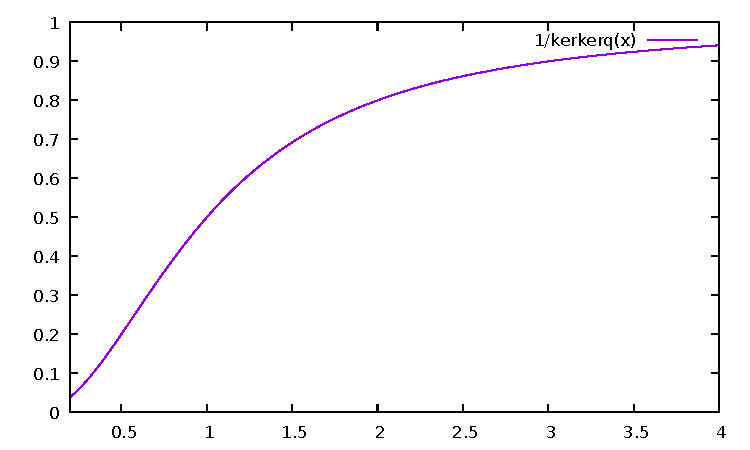
\includegraphics[width=1\linewidth]{LL1.pdf}



\end{frame}



\begin{frame}

\frametitle{Preconditioners}

My project: investigate better preconditioners than Kerker

\vspace{0.4cm}

First, a better dielectric model

\vspace{0.4cm}

\textit{New model dielectric function and exchange-correlation potential for semiconductors and insulators}
Zachary H. Levine and Steven G. Louie
Phys. Rev. B 25, 6310 1982

\vspace{0.4cm}

Still isotropic -- include anistropy?

\end{frame}



\begin{frame}

\frametitle{Preconditioners}

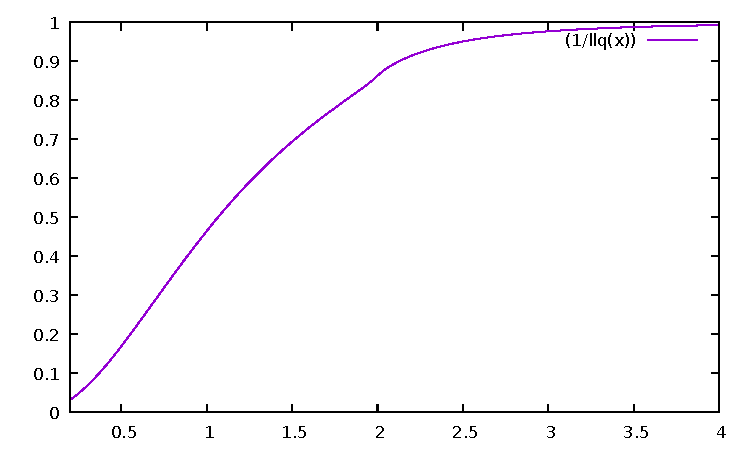
\includegraphics[width=1\linewidth]{LL.pdf}



\end{frame}


\begin{frame}

\frametitle{Preconditioners}

Both models include two parameters

\vspace{0.4cm}

How do they map onto each other?

\vspace{0.4cm}

What are the optimal parameters?

\end{frame}





%------------------------------------------------
\section{Results}
\begin{frame} 



To come...


\end{frame}

%------------------------------------------------








\end{document} 
